\section{Mapserver Peta Bali}
MapServer  adalah aplikasi freeware dan Open Source digunakan untuk  menampilkan GIS di web. Salah satunya adalah penggunaan Mapserver pada Peta Bali karena sudah tersedia pada web Mapserver. Cara menjalankan aplikasi tersebut perlu menginstall MS4W.
Mapzen dibangun dari berbagai peralatan open-source yang dikemas ke dalam layanan Web dan di hosting di server Mapzen. Salah satu keunggulan Mapzen selain keterbukaannya adalah penggunaan mesin rendering fleksibel yang disebut Tangram untuk menampilkan peta digital dalam nuansa 2D maupun 3D secara real-time, sehingga membuat kartografi akan terlihat bagus dimana-saja.
MS4W ini dapat digunakan pada windows dalam menjalan Mapserver Bali tersebut. Disini akan dijelaskan cara instalasi, proses penggunaan MapServer pada Peta Bali, dan Hasil Proses yang sudah dijalankan tersebut.
\subsection{Cara Instalasi Mapserver}
\begin{enumerate}
\item
Download Mapserver atau disingkat MS4W di http://mapserver.org/download.html \ref{gambar1} seperti gambar dibawah ini
\begin{figure}[ht]
	    \centerline{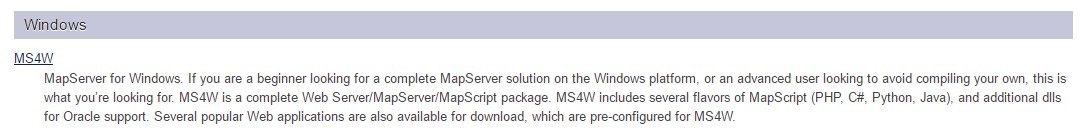
\includegraphics[width=0.50\textwidth]{figures/gambar1.JPG}}
	    \caption{Download MS4W}
		\label{gambar1}
		\end{figure}
\item
Setelah di download jalankan setupnya, disini saya menggunakan port 8080 karena port default 80 sudah dipakai oleh xampp \ref{gambar2} seperti gambar dibawah ini
\begin{figure}[ht]
	    \centerline{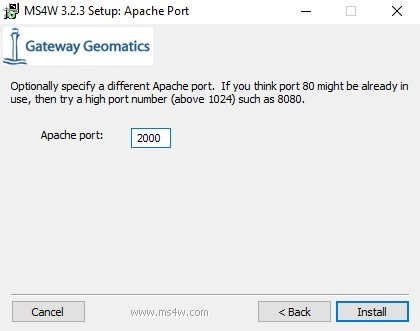
\includegraphics[width=0.50\textwidth]{figures/gambar2.JPG}}
	    \caption{Port 2000}
		\label{gambar2}
		\end{figure}
\item
Lalu tunggu instalasi sampai selesai \ref{gambar3} seperti gambar dibawah ini
\begin{figure}[ht]
	    \centerline{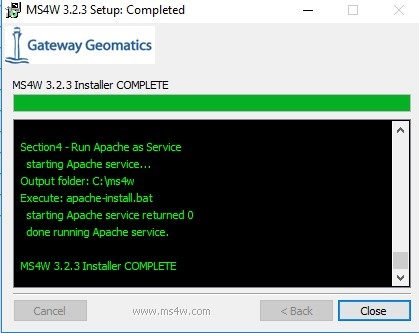
\includegraphics[width=0.50\textwidth]{figures/gambar3.JPG}}
	    \caption{Selesai}
		\label{gambar3}
		\end{figure}
\item
Setelah proses selesai silahkan buka browser favorit anda, kemudian ketikkan http://localhost:8080 di kotak isian URL.
\item
Jika anda melihat tampilan home MAPSERVER atau MS4W proses instalasi anda berhasil \ref{gambar4} seperti gambar dibawah ini
\begin{figure}[ht]
	    \centerline{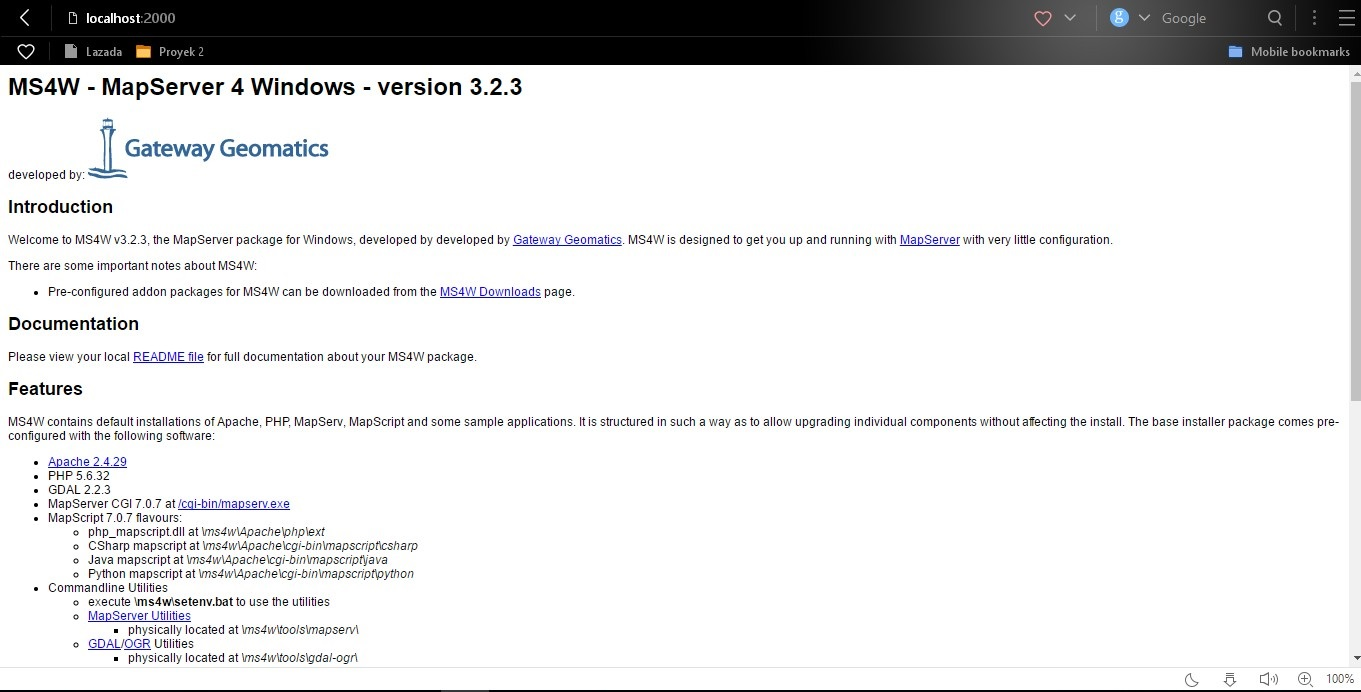
\includegraphics[width=0.50\textwidth]{figures/gambar4.JPG}}
	    \caption{Tampilan MS4W}
		\label{gambar4}
		\end{figure}
\end{enumerate}
Sekian Proses instalasi Mapserver pada Windows

\subsection{M4SW}
MS4W dilengkapi dengan berbagai modul tambahan yang mempermudah kita membangun dan mengadministrasi sistem WebGIS. Antara lain : MapLab, KaMap, Chameleon, dan lain-lain. MapLab digunakan untuk mempermudah kita membuat file konfigurasi MapServer ( *.map ) pada aplikasi WebGIS yang kita kembangkan. Sedang Chameleon adalah framework yang menyediakan berbagai class dan method yang mempermudah kita membangun interface aplikasi WebGIS yang kita kembangkan, seperti menambahkan fitur zoom, pan, dsb. Informasi mengenai MS4W, MapLab dan Chameleon dapat diperoleh di situs www.maptools.org. Di situs tersebut di dalamnya sudah terdapat aplikasi Apache Web Server, PHP, Map Server dan berbagai library yang diperlukan untuk membangun sistem WebGIS. Terdapat dua versi MS4W yang dapat didownload, versi 1.x dan versi 2.x. Akan tetapi Apabila kita akan menggunakan framework chameleon, lebih bagus pilih MS4W versi 1.x (versi 1.6) karena Chameleon belum mendukung penuh PHP5 pada paket MS4W versi 2.x.

\subsection{Arsitektur Dasar Aplikasi MapServer}
Map File - file konfigurasi teks terstruktur untuk aplikasi MapServer Anda. Ini mendefinisikan area peta Anda, memberi tahu program MapServer tempat data Anda berada dan di mana menampilkan gambar.
Data Geografis - MapServer dapat memanfaatkan banyak jenis sumber data geografis. Format defaultnya adalah format ESRI Shape.
HTML Pages - antarmuka antara pengguna dan MapServer. Mereka biasanya duduk di root Web. Dalam bentuknya yang paling sederhana, MapServer dapat dipanggil untuk menempatkan gambar peta statis pada halaman HTML. Untuk membuat peta interaktif, gambar ditempatkan dalam bentuk HTML pada halaman.
MapServer CGI - File biner atau executable yang menerima permintaan dan mengembalikan gambar, data, dan lain-lain. Ini ada di direktori cgi-bin atau script dari server web.
Web / HTTP Server - menyajikan halaman HTML saat dilanda browser pengguna.

\begin{table}[h]
\caption{Paket dasar M4SW}
\centering
\begin{tabular}{cc}
\hline
1&Webserver Apache\\
\hline
2&PHP\\
\hline
3&MapServer CGI\\
\hline
4&PHP/Mapscript\\
\hline
5&Program utiliti (pustaka) GDAL dan OGR\\
\hline
6&Program utiliti MapServer (shp2img, legend, scalebar, sortshp, sym2img, shptree, dan tile4ms)\\
\hline
7&Ekstensi OGR/PHP\\
\hline
8&OWTChart\\
\hline
\end{tabular}
\end{table}
